\def\CC{{C\nolinebreak[4]\hspace{-.05em}\raisebox{.4ex}{\tiny\bf ++}}}
%
%======================================================================
%======================================================================
%======================================================================
\begin{frame}{Why Entropy-stable DG}
	\begin{itemize}
		\setlength{\itemsep}{0.2in}
		\item  Challenge:  Shock Capturing DG is dissipative, which damps small scales and lowers the fidelity of turbulence simulations 
		\item  Entropy stable:
		\begin{itemize}
			\item Exact governing equation also implies an entropy condition
			\item Standard DG only does this approximately
			\item Make the discretization also strictly obey the entropy condition
			\item Less numerical dissipation is better for turbulence simulation and shock capturing
		\end{itemize}
		\item Mathematical interpretation:
		\begin{itemize}
			\item Additional constraint singles out the ``right'' solution when characteristic waves intersect
			\item The resulting symmetric hyperbolic system is formally well posed
		\end{itemize}
	\end{itemize}
\end{frame}
%======================================================================

%======================================================================
%======================================================================
\begin{frame}{ES on continuous cases}
	\begin{itemize}
		\item The convex entropy function for CNS is \[U = -\rho s/(\gamma-1);\quad s = ln(p\rho^{-\gamma})\]
		\item The entropy variables ${\bf v} = \frac{\partial U}{\partial{\bf Q}}$.
		
		\item Entropy potential \[\psi_i({\bf v}) = {\bf v}^Tf_i({\bf Q}({\bf v})) -F_i({\bf Q}({\bf v})),\quad 1\leq i\leq d\]
		In CNS $\psi = \sum_{i=1}^d\psi_i = \sum_{i=1}^d\rho u_i$
		\item The entropy conservative/stable flux $\widetilde{f}_S$ is defined as \[({\bf{v}}_L-{\bf{v}}_R)^T\widetilde{\bf{f}}_S({\bf{Q}}_L,{\bf{Q}}_R)\leq\psi_i({\bf{Q}}_L)-\psi_i({\bf{Q}}_R)\]
	\end{itemize}
\end{frame}
\begin{frame}{Keys for ES in discrete level}
	\begin{itemize}
		\item Using entropy stable bi-variate flux with the correct amount of entropy dissipation at each interface. 
		
		\item Using flux differencing techniques
		\begin{itemize}
			\item Continuum:
			\[(\widetilde{{\bf f}}_S, \frac{\partial{\bf v}}{\partial x})_{T_\kappa} = (\frac{\partial{\boldsymbol \psi}}{\partial x},{\bf 1})_{T_{\kappa}}\]
			\item Discretely: \[({\bf v}^k)^T{\bf D}^k{\bf W}\widetilde{{\bf f}}_n^k\neq ({\boldsymbol{\psi}}_n^k)^T{\bf D}^k{\bf W}{\bf 1}^k \]
		\end{itemize}
		\item Differentiate at both volume and surface (Hybridized operator is recommended)
	\end{itemize}
\end{frame}
%======================================================================
\begin{frame}\frametitle{Governing Equation \& Example}
	\begin{itemize}
		\item Navier-Stokes: 
		\begin{equation*}
			\frac{\partial{\bf{Q}}}{\partial{t}}+\frac{\partial({{\bf f}_i({\bf Q})}-{\bf g}_i({\bf Q}))}{\partial{x}} = 0,\quad(\textbf{x},t)\in \mathbb{R}^d \times [0,\infty)
		\end{equation*}
		\begin{equation*}
			{\bf Q} = \big[\rho, \rho u, \rho E\big]^T
		\end{equation*}
		\begin{equation*}
			\quad {\bf f}({\bf Q}) = \big[\rho u, \rho u^2+p, u(\rho{E}+p)\big]^T
		\end{equation*}
		\begin{equation*}
			\quad {\bf g}({\bf Q}) = \bigg[0, \tau_{1,1}, u\tau_{1,1}-\kappa\frac{\partial{T}}{\partial{x}}\bigg]^T 
                      \end{equation*}
                    \item 
		Shu-Osher shock tube: {\begin{equation*}
			\begin{bmatrix}
				\rho(x) \\
				u(x) \\
				p(x)
			\end{bmatrix} = 
		\begin{bmatrix}
			3.8571 \\
			2.6293 \\
			10.333
		\end{bmatrix} (x\leq0.125)\quad
	\begin{bmatrix}
		\rho(x) \\
		u(x) \\
		p(x)
	\end{bmatrix} = 
	\begin{bmatrix}
		1+0.2\sin(16\pi x) \\
		0 \\
		1
	\end{bmatrix} (\text{else})
		\end{equation*}}
	\end{itemize}
\end{frame}

\begin{frame}\frametitle{1D Demonstration:  Stable w/o Viscosity}
	\begin{itemize}
	
		\item Discretization: $p=3$ (degree), $K = 300$ (elements)
		\item Viscosity: ESDG $\mu = 0$, Standard DG $\mu = 3\times 10^{-3}$ (needed for stability)
                \item DG dissipation damps features \ldots
                \end{itemize}
                \medskip
                \begin{center}
                          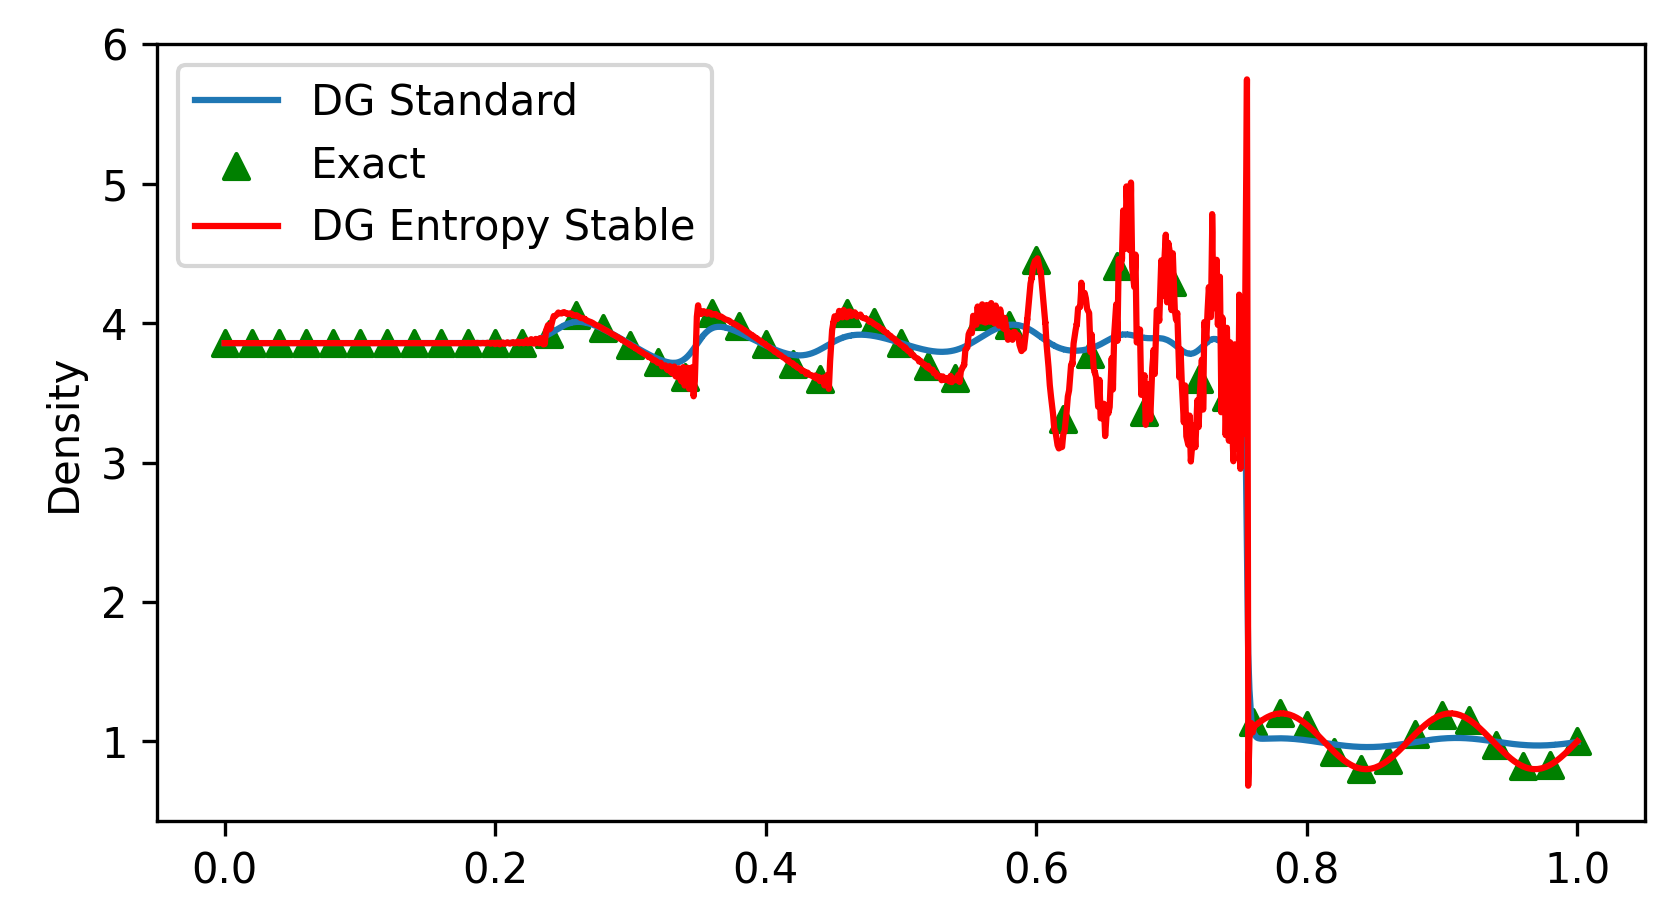
\includegraphics[width=0.6\linewidth]{figures/RHO.png}          
	\end{center}
        \centerline{\iPI{Does not need turbulence-harmful dissipation to be stable!}}
\end{frame}

\begin{frame}{Current Work}
	\begin{itemize}
		\setlength{\itemsep}{0.2in}
		\item  1D+ testing implementation for toy problems and quick testing
		\item  Now using: implementation in \textit{MIRGE-Com} (Zirui up next!)
		\item Analyze:
		\begin{itemize}
			\item Turbulence spectra using DNS
			\item The dispersion relation for entropy stable scheme using linearized case
		\end{itemize}
	\end{itemize}
      \end{frame}


\begin{frame}\frametitle{Status of ESDG in \mirgecom{}}
\vspace{15pt}
\begin{center}
\mirgecom{} ESDG branch: https://github.com/illinois-ceesd/mirgecom@production-esdg
\end{center}
%\begin{multicols}{2}
\begin{itemize}
% \item Implementation status
%\begin{itemize}
\item Work of Thomas Gibson modernized (grudge, mirgecom)
\item ESDG-enabled RHS operators in \mirgecom{}:
\begin{itemize}
\item Euler
\item CNS with ESDG for inviscid terms only
\end{itemize}
\item Exercises and tests:
\begin{itemize}
\item Selected \mirgecom{} example drivers
\item Prediction driver
\end{itemize}
\end{itemize}
%\item Using ESDG in \mirgecom{}
%\begin{itemize}
%\item Driver update
%\item Examples
%\end{itemize}
%\end{itemize}
%\item Troubles
%\begin{itemize}
%\item Multicomponent diffusion (advection ok)
%\item Prediction boundary issue
%\end{itemize}
%\item Can be improved...
%\end{itemize}
%\columnbreak
%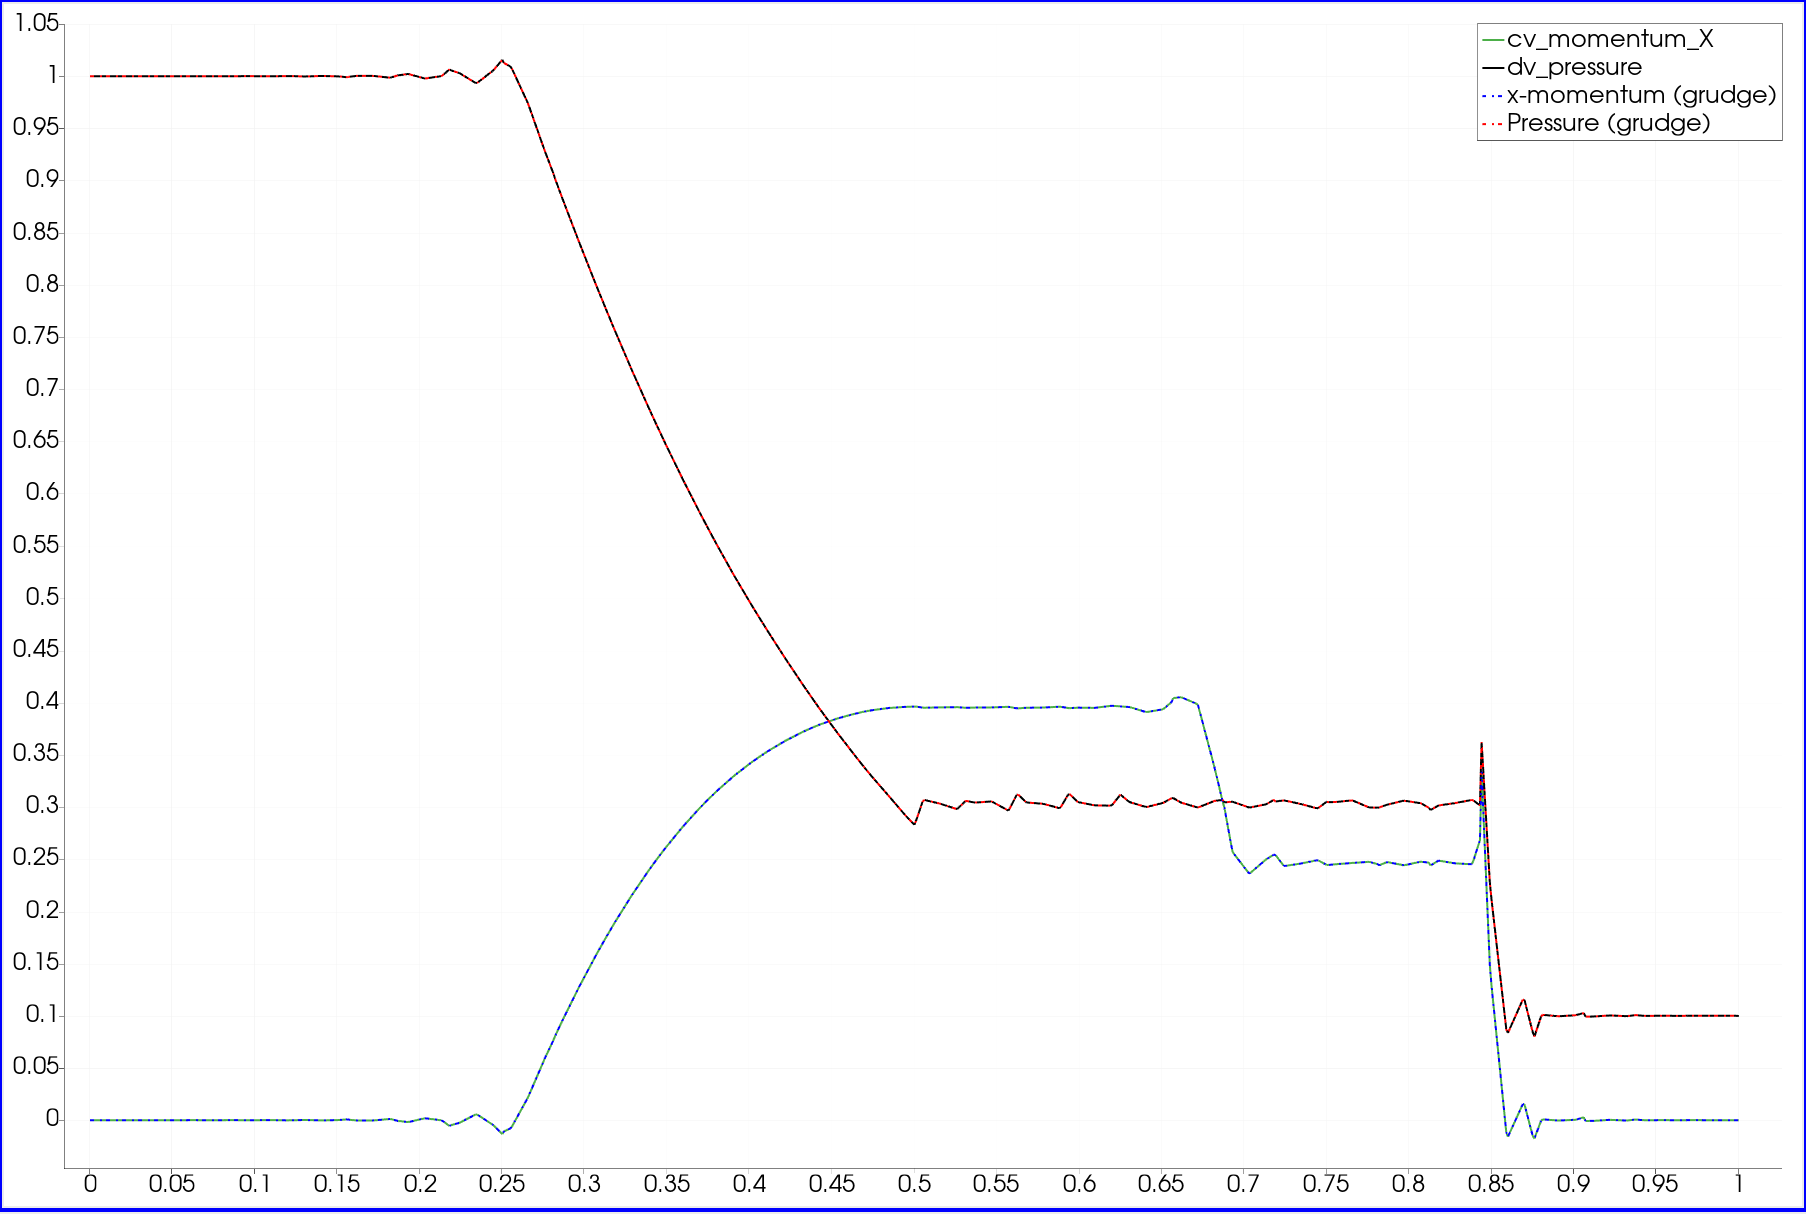
\includegraphics[width=.48\textwidth]{figures/compare-sod-shock-esdg-grudge.png}
%\end{multicols}
\end{frame}

\begin{frame}[fragile]\frametitle{ESDG Procedure in \mirgecom{}}
\begin{multicols}{2}
\begin{itemize}
\setlength{\itemsep}{3pt}
\item Project fluid conserved variables ($\mathbf{Q}$) to quadrature points $\rightarrow\mathbf{Q}_q$
\item Calculate Entropy Variables ($\mathbf{V}$) from projected $\mathbf{Q}_q$
\item Project $\mathbf{V}$ to element boundaries $\rightarrow$ $\mathbf{V}_b$ (communicate too)
\item Compute modified $\mathbf{Q}$ from $(\mathbf{V},\mathbf{V}_b) \rightarrow (\tilde{\mathbf{Q}},\tilde{\mathbf{Q}}_b)$
\item Flux $\tilde{\mathbf{Q}}$ using
\begin{itemize}
\item usual BCs with $\tilde{\mathbf{Q}}_b$
\item entropy-conserving flux routines
\end{itemize}
\item Hit with DG div operator for RHS
\end{itemize}
\columnbreak
\begin{center}
entropy\_stable\_euler\_operator
\end{center}
\vspace{-10pt}
\begin{lstlisting}
# Interpolate state to vol quad grid
cv_q = project_fluid_state(vol, quad, state)

# Compute the projected (nodal) entropy variables
ev = volume_quadrature_project(
      quad,
      # Map to entropy variables
      conservative_to_entropy_vars(gamma, cv_q)
     )

# Makes [vol, surf] two-point flux-ready array
cv_prime = \
  make_entropy_projected_fluid_state(
     vol, faces, cv, ev)

# EC volume flux for CV'
flux_matrices = \
   entropy_conserving_flux_chandrashekar(
      gas_model, cv_prime))

# Compute volume derivatives using flux differencing
vol_term = \
  -volume_flux_differencing(quad, faces_quad,
                            flux_matrices)

# CV' on interior faces
cv_mod_interior_pairs = [
  _interp_modified_cv(gamma, tpair)
  for tpair in interior_trace_pairs(dcoll, ev)
]

# CV' on domain bnd
domain_bnd_states = {
  btag: project_fluid_state(
    dcoll, dd_vol,
    as_dofdesc(btag).with_discr_tag(quadrature_tag),
    cv, entropy_stable=True)
    for btag in boundaries
}

# Compute interface contributions
flux_bnd = \
  inviscid_flux_on_element_boundary(
    dcoll, gas_model, boundaries, cv,
    domain_bnd_states)

# RHS = div(ec-fluxes) 
return div_operator(vol_term, flux_bnd)

\end{lstlisting}
\end{multicols}
% Note: uses native mirgecom boundaries, but with CV' and EC fluxes
\end{frame}

\begin{frame}[fragile]
  \frametitle{Using ESDG in \mirgecom{}}
  \begin{minipage}[b]{0.48\textwidth}
    \begin{itemize}
      \item Install \mirgecom{} ESDG branch
      \item Update \mirgecom{} driver
      \begin{itemize}
        \item Import ESDG operators
        \item Overintegration required (default order$~=\!2p\!+\!1$)
        \item ESDG is lazy-only
      \end{itemize}
    \end{itemize}
  \end{minipage}\hfill
  \begin{minipage}[b]{0.48\textwidth}
    \centering
\begin{lstlisting}
from mirgecom.euler import (
   euler_operator, entropy_stable_euler_operator
)
from mirgecom.navierstokes import (
   ns_operator, entropy_stable_ns_operator
)
from grudge.dof_desc import DISCR_TAG_QUAD
\end{lstlisting}
    % 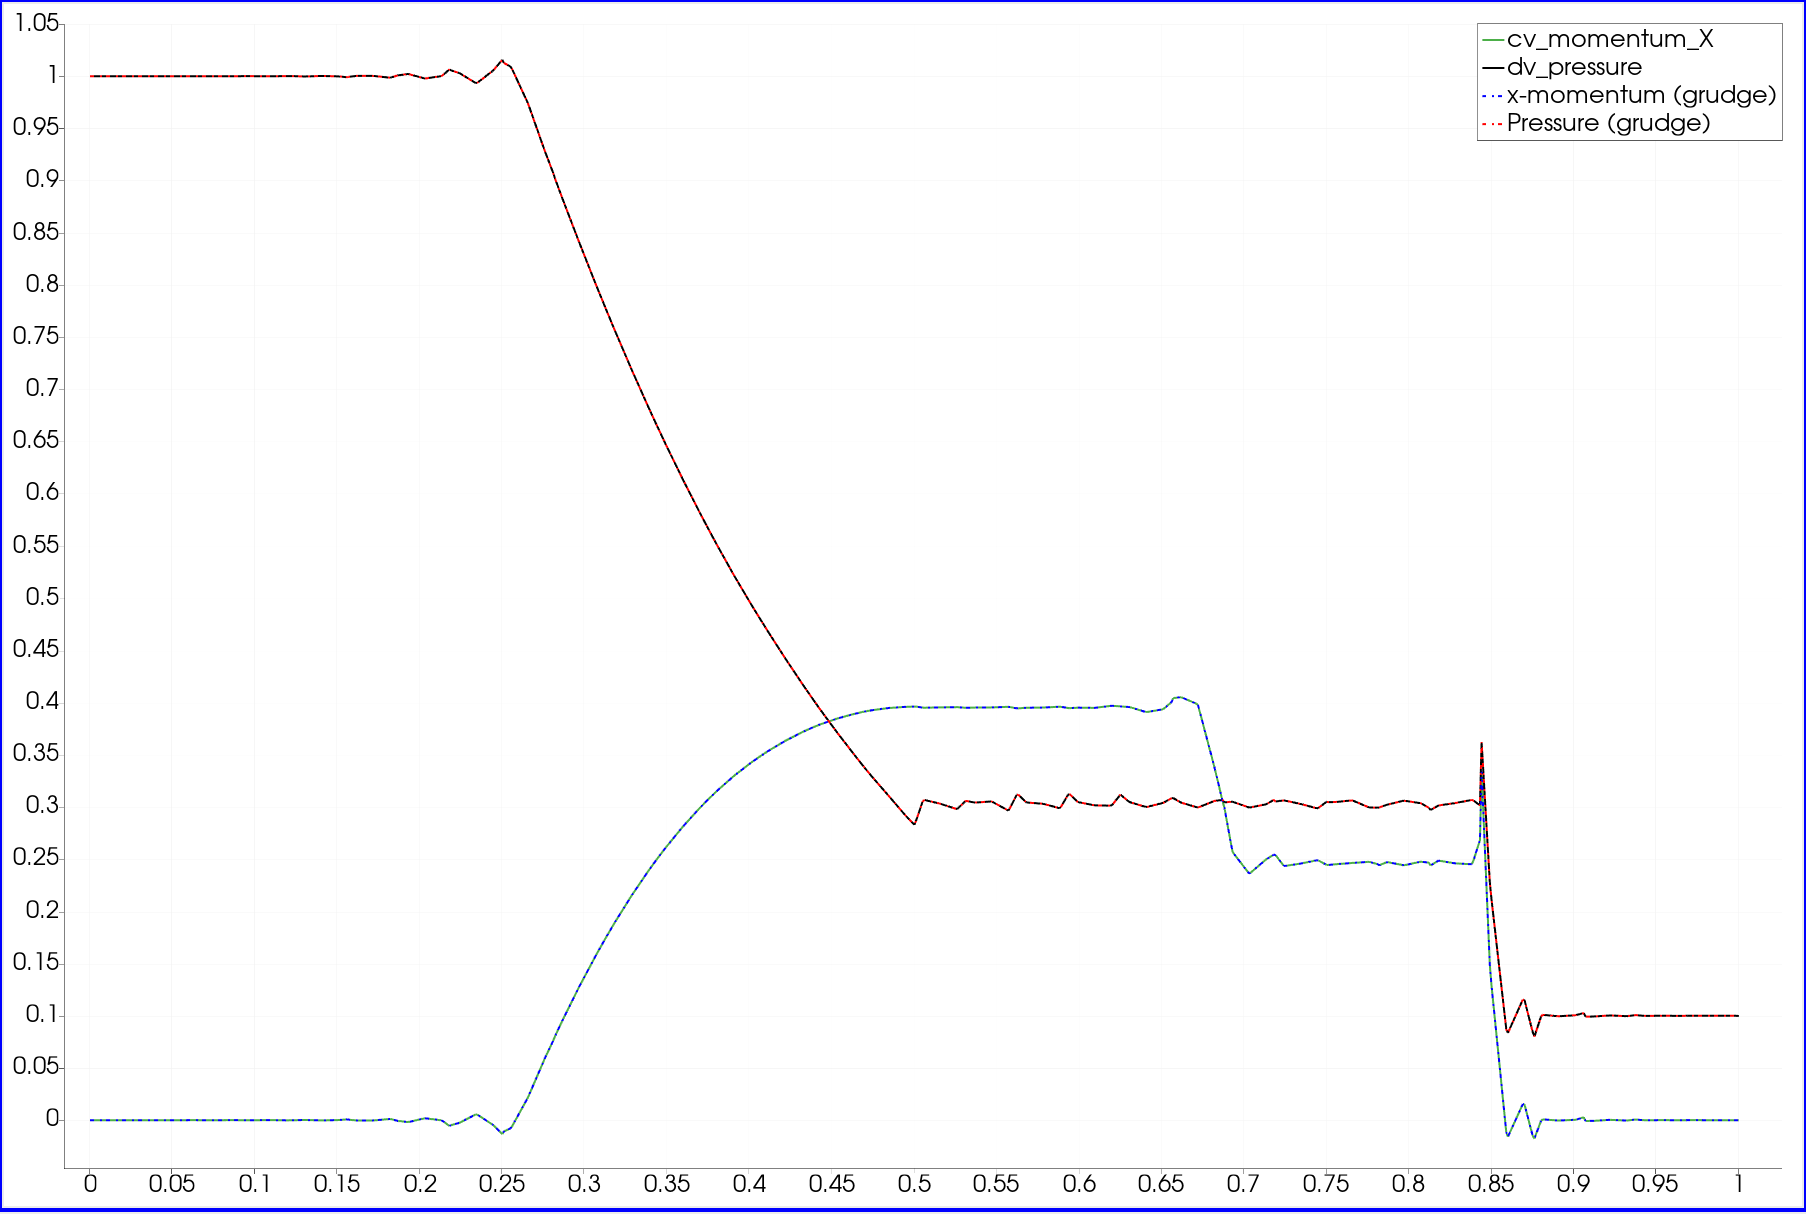
\includegraphics[width=\textwidth]{figures/compare-sod-shock-esdg-grudge.png}
    % \vspace{5pt} % adjust as needed
    \tiny Import the appropriate operator for the case, and the \textit{grudge} quadrature tag
\begin{lstlisting}
# 2 times element order (+1?)
q_tag = DISCR_TAG_QUAD
q_ord = 2 * p
dcoll = \
  create_discretization_order(
     lazy_actx, mesh, order=p,
     quadrature_order=q_ord)

def my_rhs(t, state):
  return entropy_stable_ns_operator(
          state, t, ..., quadrature_tag=qtag)
\end{lstlisting}
    % 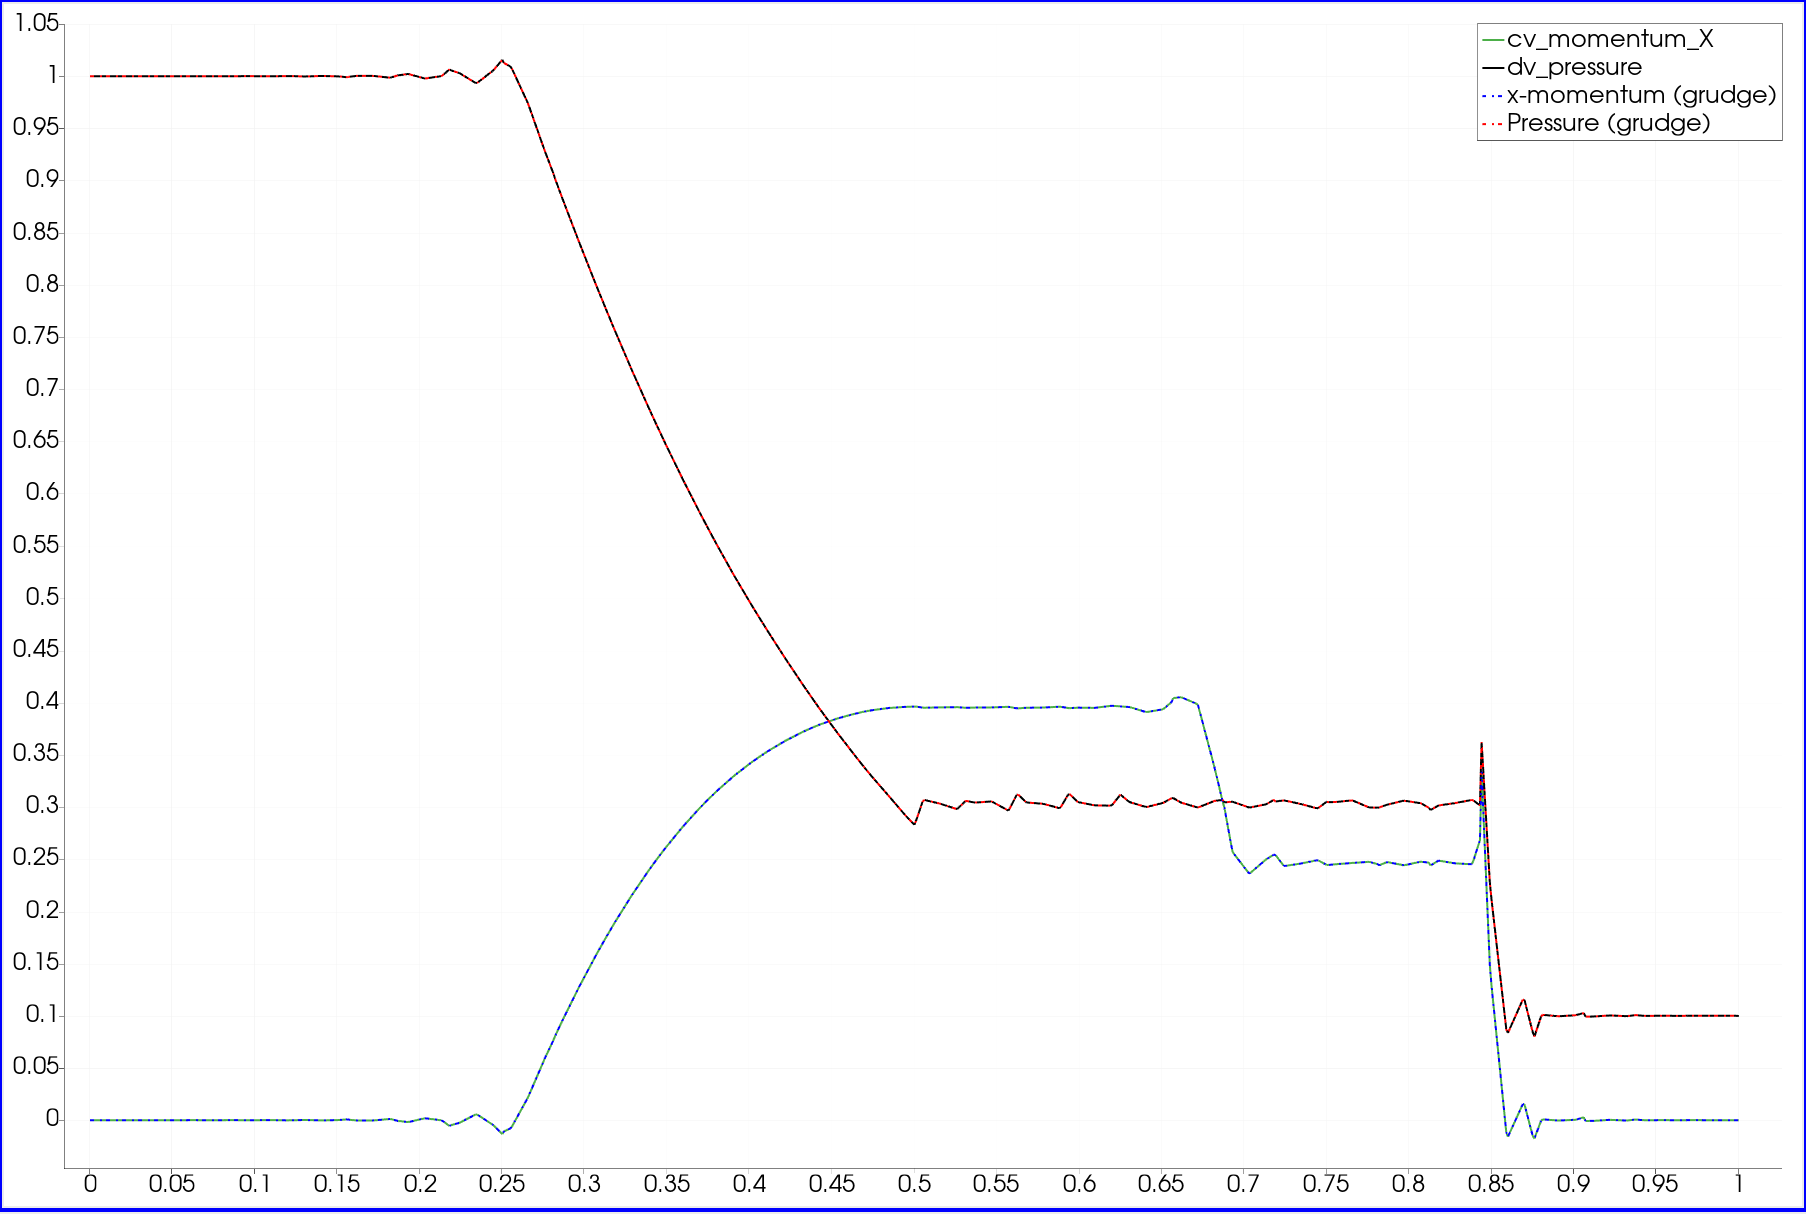
\includegraphics[width=\textwidth]{figures/compare-sod-shock-esdg-grudge.png}
    % \vspace{5pt} % adjust as needed
    \tiny Set the quadrature order and \texttt{quadrature\_tag}. Pass \texttt{quadrature\_tag} to ESDG operator.
  \end{minipage}
\end{frame}

\begin{frame}
  \frametitle{ESDG Examples in \mirgecom{}}
  \begin{minipage}[b]{0.48\textwidth}
        \begin{itemize}
        \item sod-mpi.py
        \item pulse-mpi.py
        \item vortex-mpi.py
        \item taylor-green-mpi.py
        \item poieuille-mpi.py
        \item combozzle-mpi.py
        \item thermally-coupled-mpi.py
        \end{itemize}
  \end{minipage}\hfill
  \begin{minipage}[b]{0.48\textwidth}
    \centering
    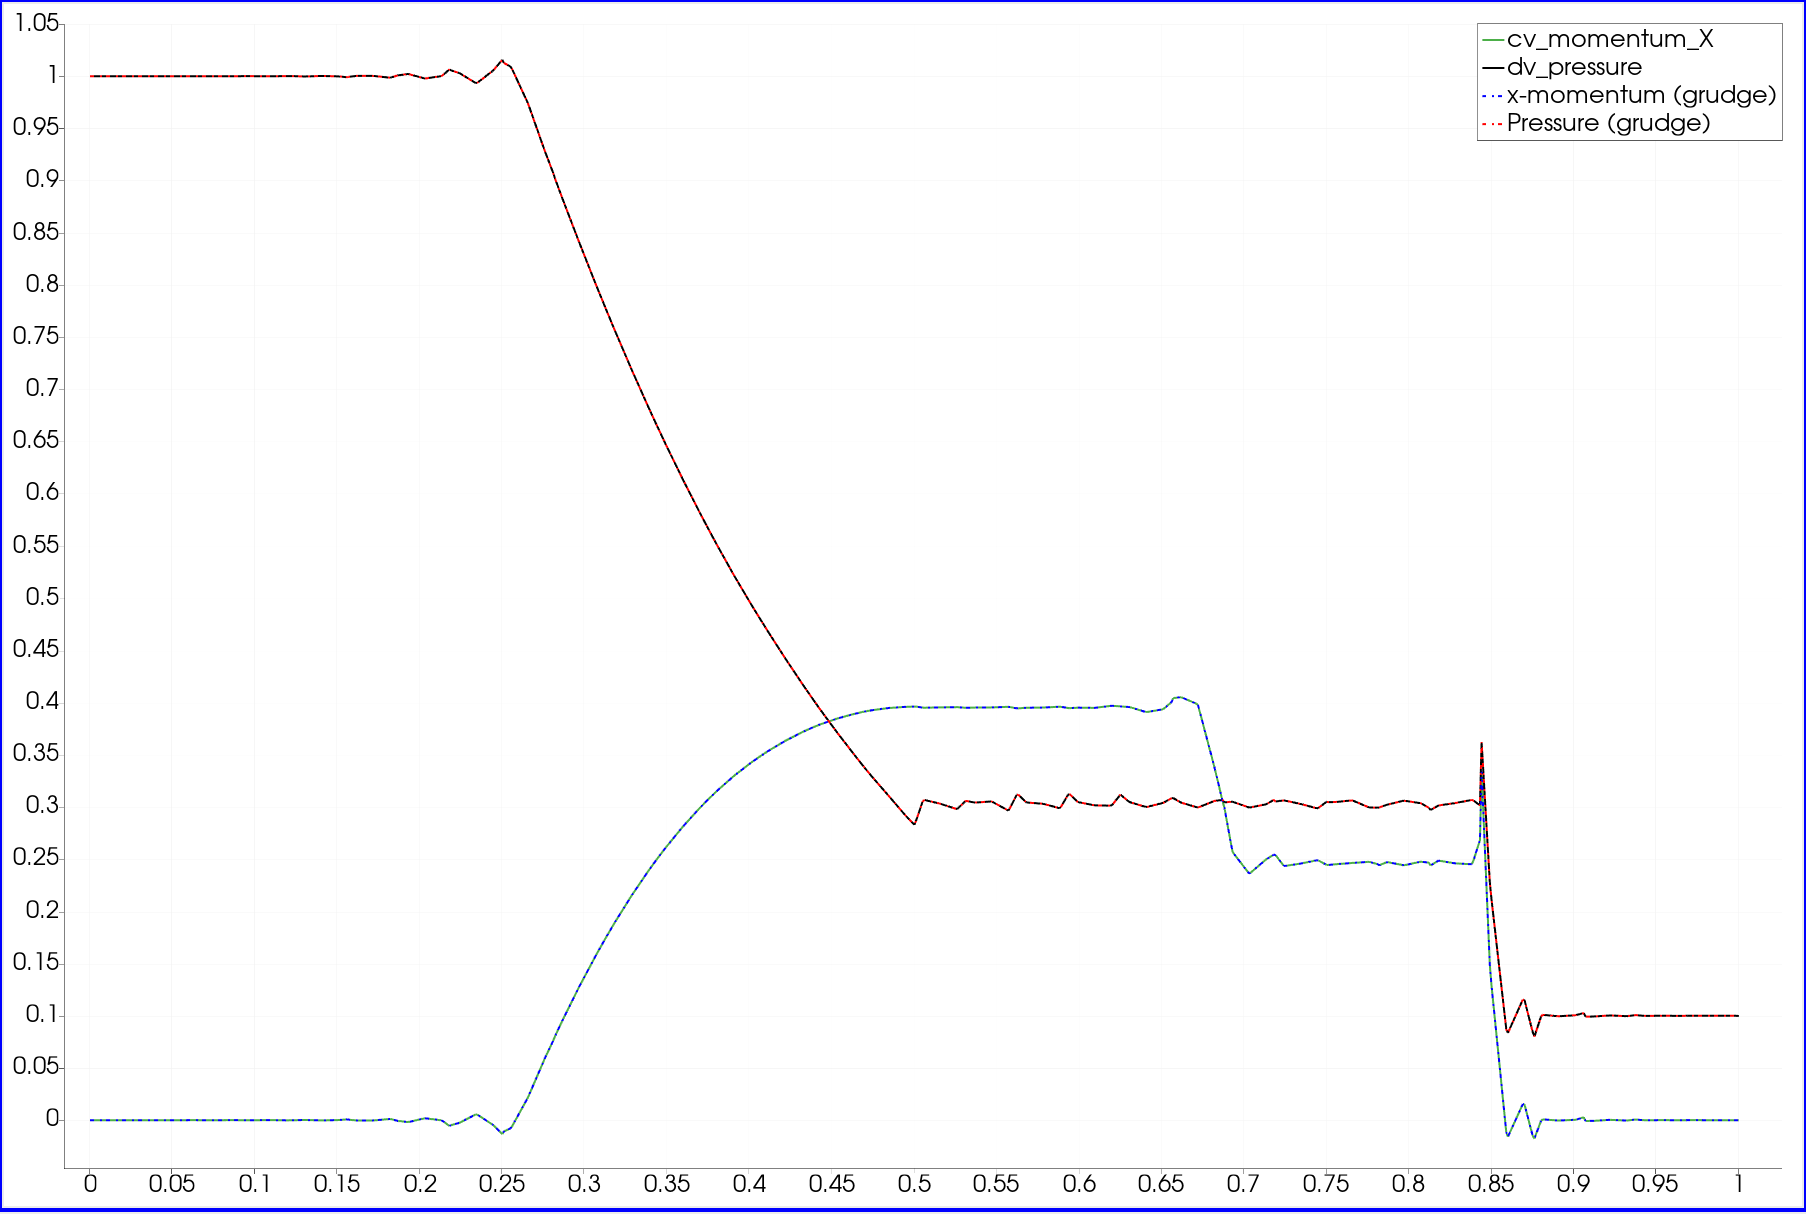
\includegraphics[width=\textwidth]{figures/compare-sod-shock-esdg-grudge.png}
    \vspace{5pt} % adjust as needed
    \footnotesize 1D Sod Shock Tube example in \mirgecom{}. Results match \textit{grudge} for $32~~p\!=\!4$ cells. Standard DG crashes on this case.
  \end{minipage}
\begin{center}
%\begin{lstlisting}
    \begin{tcolorbox}[colback=white,colframe=black,width=\textwidth,
                      boxrule=0.5pt,left=0pt,right=0pt,top=0pt,bottom=0pt]
      \footnotesize\texttt{python -m mpi4py <driver\_name>.py ----esdg [-----overintegration ----lazy]}
    \end{tcolorbox}
%\texttt{python -m mpi4py <driver\_name>.py ----esdg [-----overintegration ----lazy]}
%\end{lstlisting}
\end{center}  
\end{frame}

%\begin{frame}
%  \frametitle{Using ESDG in \mirgecom{}}
%  \begin{minipage}[b]{0.48\textwidth}
%    \begin{itemize}
%      \item Install \mirgecom{} ESDG branch
%      \item Update \mirgecom{} driver
%      \begin{itemize}
%        \item ESDG is lazy-only
%        \item Use Overintegration (default order$~=\!2p\!+\!1$)
%        \item Use ESDG operators
%      \end{itemize}
%      \item Examples:
%      \begin{itemize}
%        \item sod-mpi.py
%        \item pulse-mpi.py
%        \item vortex-mpi.py
%        \item taylor-green-mpi.py
%        \item poieuille-mpi.py
%        \item combozzle-mpi.py
%        \item thermally-coupled-mpi.py
%      \end{itemize}
%    \end{itemize}
%  \end{minipage}\hfill
%  \begin{minipage}[b]{0.48\textwidth}
%    \centering
%    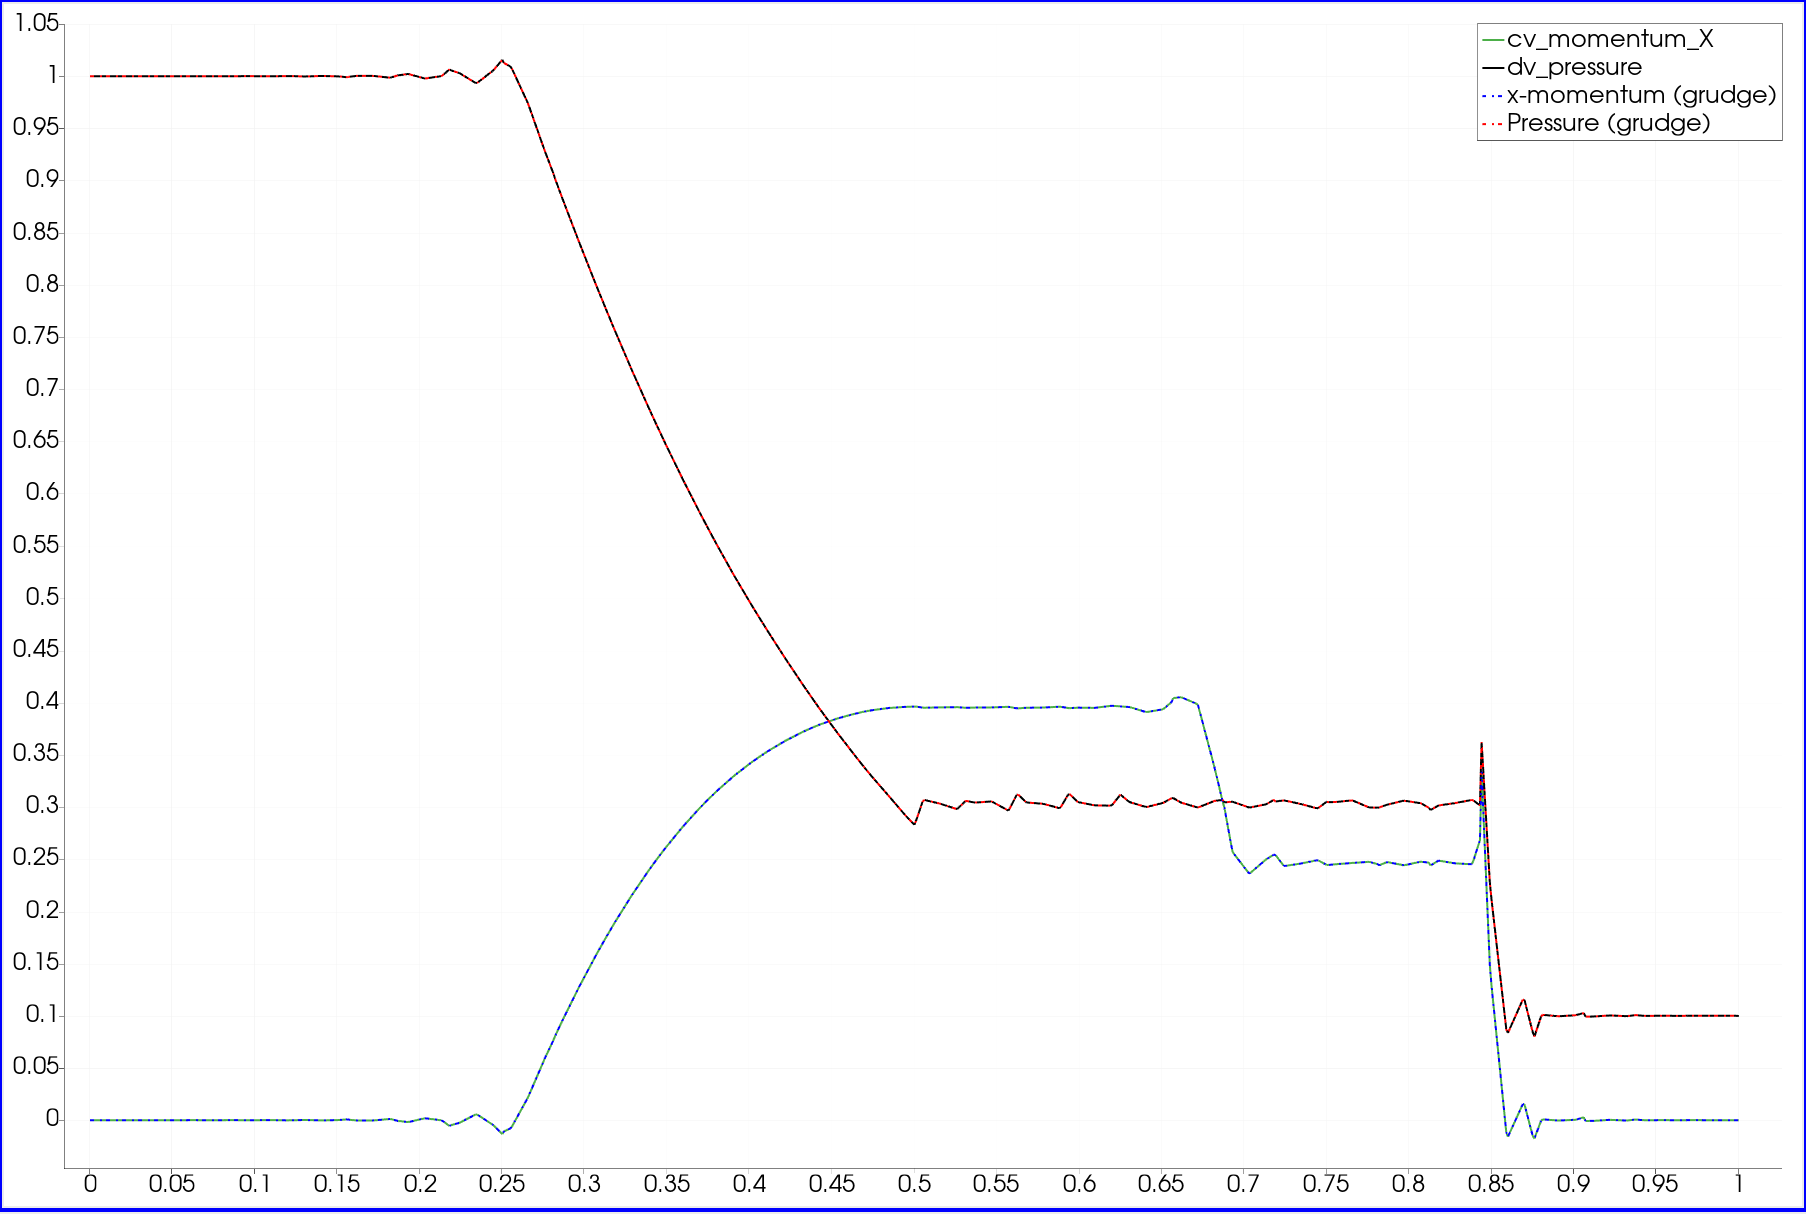
\includegraphics[width=\textwidth]{figures/compare-sod-shock-esdg-grudge.png}
%    \vspace{5pt} % adjust as needed
%    \footnotesize 1D Sod Shock Tube example in \mirgecom{}. Results match \textit{grudge} for $32~~p\!=\!4$ cells. Regular ol' DG crashes on this case.
%  \end{minipage}
%\end{frame}

\begin{frame}
  \frametitle{Status of ESDG in Prediction}
  \begin{minipage}[b]{0.48\textwidth}
      \begin{itemize}
      \item Prediction-related code updates:
        \begin{itemize}
        \item \mirgecom{} PR\#877
        \item \textit{drivers\_y3-prediction} PR\#26
        \end{itemize}
      \item Currently making nans near the isothermal noslip boundaries
      \item Debugging
        \begin{itemize}
        \item Runs multiphysics example without issue
        \item Running Poiseuille isothermal noslips without issue 
        \item Will use Shock1D to debug more
        \end{itemize}
      \end{itemize}
  \end{minipage}\hfill
  \begin{minipage}[b]{0.48\textwidth}
    \centering
    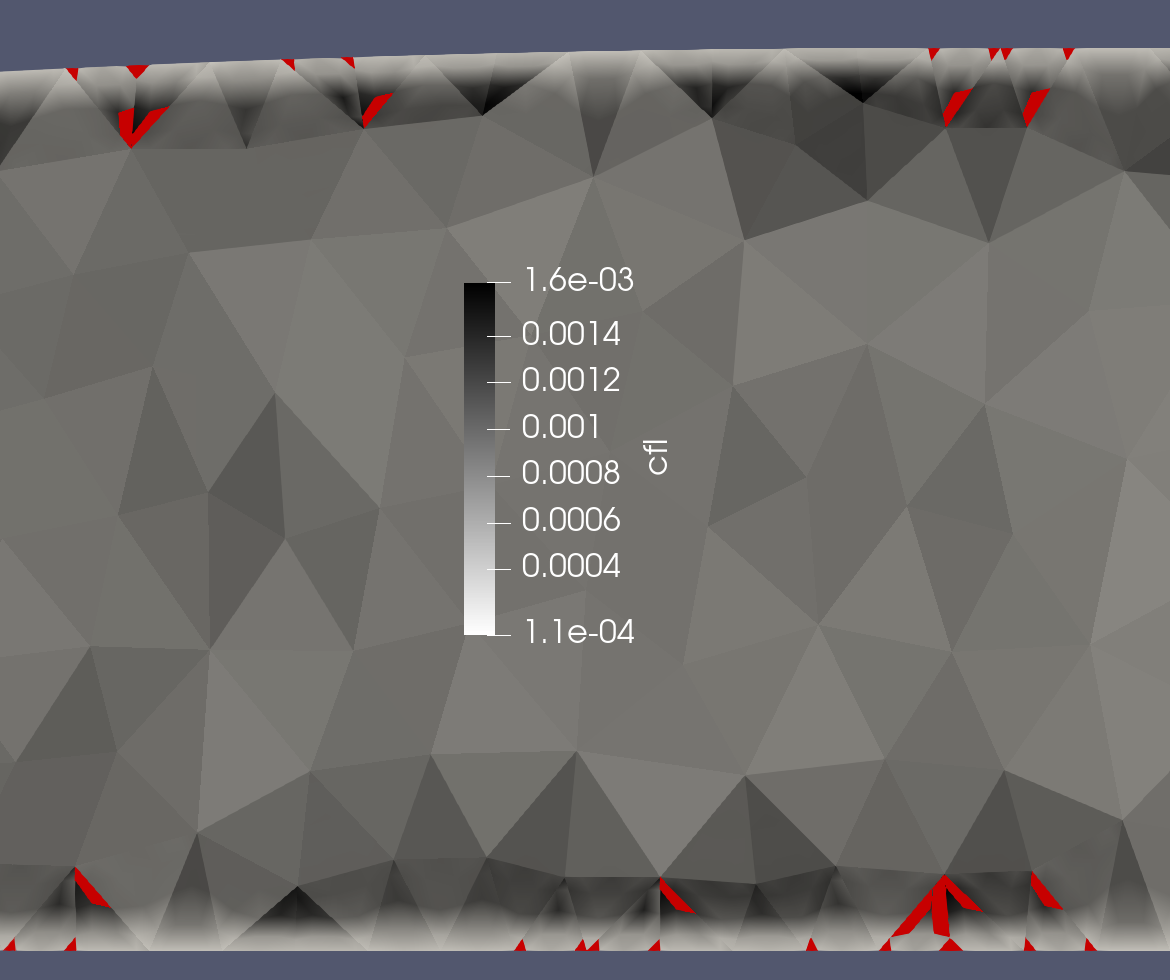
\includegraphics[width=.9\textwidth]{figures/prediction-esdg-nans.png}
    % 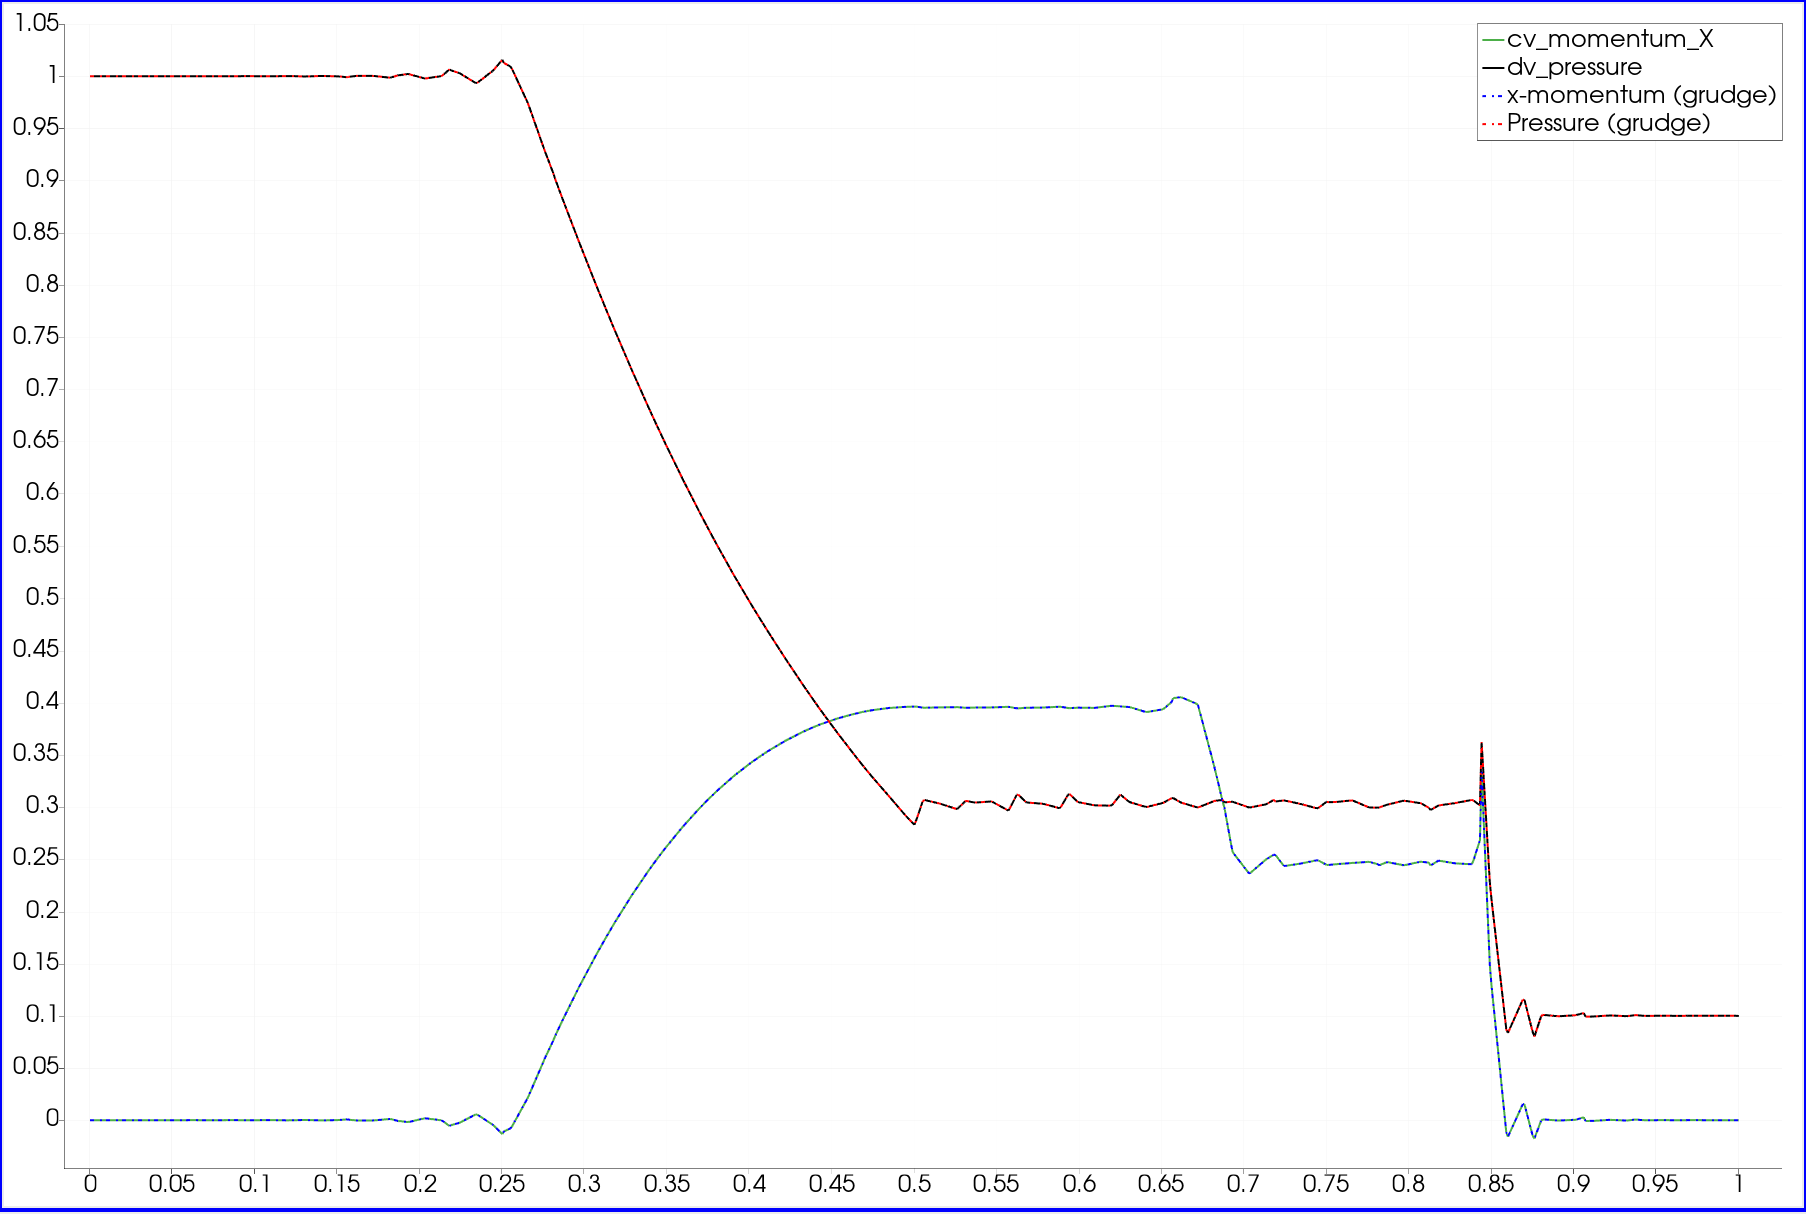
\includegraphics[width=\textwidth]{figures/compare-sod-shock-esdg-grudge.png}
    \vspace{5pt} % adjust as needed
    \footnotesize \textit{drivers\_y3-prediction} 2D smoke test, single gas. ESDG gets NaNs right away.
    % \footnotesize 1D Sod Shock Tube example in \mirgecom{}. Results match \textit{grudge} for $32~~p\!=\!4$ cells. Regular ol' DG crashes on this case.
  \end{minipage}
\end{frame}

\begin{frame}\frametitle{What's next for ESDG?}
\begin{itemize}
\item Prediction w/ESDG is then main priority, then ...
\item Eliminate the glued-together vol/surf construction in grudge
\item Better integration with the native operators
\item Fix bugs in multi-component, and mixtures cases:
\begin{itemize}
\item Scalar advection OK
\item Scalar diffusion not OK
\end{itemize}
\item Analysis: Do we need to extend ESDG to include viscous terms?
\end{itemize}
\end{frame}
